\documentclass[11pt,a4paper]{article}

% Packages
\usepackage[utf8]{inputenc}
\usepackage[T1]{fontenc}
\usepackage{geometry}
\usepackage{graphicx}
\usepackage{booktabs}
\usepackage{array}
\usepackage{longtable}
\usepackage{float}
\usepackage{xcolor}
\usepackage{hyperref}
\usepackage{amsmath}
\usepackage{amssymb}
\usepackage{caption}
\usepackage{subcaption}
\usepackage{fancyhdr}
\usepackage{titlesec}
\usepackage{enumitem}

% Page geometry
\geometry{margin=2.5cm}

% Colors
\definecolor{tier1}{HTML}{00D4AA}
\definecolor{tier2}{HTML}{FFB800}
\definecolor{tier3}{HTML}{FF4757}
\definecolor{primaryblue}{HTML}{4A90D9}

% Header/Footer
\pagestyle{fancy}
\fancyhf{}
\fancyhead[L]{GNSS Sensor Deep Analysis Report}
\fancyhead[R]{\thepage}
\fancyfoot[C]{Confidential - Internal Use Only}

% Hyperref settings
\hypersetup{
    colorlinks=true,
    linkcolor=primaryblue,
    filecolor=magenta,
    urlcolor=cyan,
}

% Title formatting
\titleformat{\section}{\Large\bfseries\color{primaryblue}}{\thesection}{1em}{}
\titleformat{\subsection}{\large\bfseries}{\thesubsection}{1em}{}

\begin{document}

% Title Page
\begin{titlepage}
    \centering
    \vspace*{2cm}

    {\Huge\bfseries GNSS Sensor Deep Analysis Report\\[0.5cm]}
    {\Large Three-Dimensional Core Analysis\\[2cm]}

    \rule{\textwidth}{1pt}\\[0.5cm]

    {\large
    \textbf{Analysis Dimensions:}\\[0.3cm]
    1. Vertical Precision Tiering\\
    2. Environmental Coupling Analysis\\
    3. Diurnal Cycle \& Multipath Detection\\[1cm]
    }

    \rule{\textwidth}{1pt}\\[2cm]

    {\large
    \textbf{Dataset:} sensor\_data\_clean\_stable.csv\\[0.3cm]
    \textbf{Devices Analyzed:} 8\\[0.3cm]
    \textbf{Total Records:} 135,168\\[0.3cm]
    \textbf{Time Range:} 2025-11-10 to 2025-11-26\\[2cm]
    }

    \vfill

    {\large Report Generated: \today}

\end{titlepage}

% Table of Contents
\tableofcontents
\newpage

% Executive Summary
\section{Executive Summary}

This report presents a comprehensive three-dimensional analysis of GNSS sensor performance data collected from 8 devices over a 16-day period. The analysis focuses on vertical positioning accuracy, environmental factor coupling, and temporal patterns that may indicate multipath interference.

\subsection{Key Findings}

\begin{itemize}[leftmargin=*]
    \item \textbf{Vertical Precision:} All 8 devices (100\%) fall into Tier 3 (Warning) category with altitude STD $>$ 5m. No devices achieved high-precision status.

    \item \textbf{Environmental Coupling:} Weak or anomalous altitude-pressure correlations detected across all devices, suggesting potential sensor calibration issues or environmental interference.

    \item \textbf{Multipath Effects:} Significant 24-hour periodic patterns observed with diurnal amplitudes ranging from 11.17m to 21.68m, indicating probable multipath interference from nearby reflective surfaces.
\end{itemize}

\subsection{Recommendations}

\begin{enumerate}
    \item Investigate antenna installation environments for reflective surfaces
    \item Consider implementing RTK/PPP differential corrections
    \item Flag device \texttt{1878250224} for hardware inspection (903m altitude range anomaly)
    \item Implement data quality filtering for outliers beyond 3$\sigma$
\end{enumerate}

\newpage

% Dimension 1: Vertical Precision Tiering
\section{Dimension 1: Vertical Precision Tiering}

\subsection{Methodology}

Vertical precision is assessed by calculating the standard deviation (STD) of MSL altitude measurements for each device. Devices are classified into three tiers based on precision thresholds:

\begin{table}[H]
\centering
\caption{Precision Tier Definitions}
\begin{tabular}{llll}
\toprule
\textbf{Tier} & \textbf{Classification} & \textbf{Threshold} & \textbf{Application} \\
\midrule
\textcolor{tier1}{Tier 1} & High Precision & STD $\leq$ 1.5m & Survey-grade applications \\
\textcolor{tier2}{Tier 2} & Standard & STD $\leq$ 5.0m & Navigation \& tracking \\
\textcolor{tier3}{Tier 3} & Warning & STD $>$ 5.0m & Requires investigation \\
\bottomrule
\end{tabular}
\end{table}

\subsection{Results}

\begin{table}[H]
\centering
\caption{Device Precision Tier Distribution}
\begin{tabular}{lccc}
\toprule
\textbf{Tier} & \textbf{Device Count} & \textbf{Percentage} & \textbf{Status} \\
\midrule
Tier 1 (High) & 0 & 0.0\% & -- \\
Tier 2 (Standard) & 0 & 0.0\% & -- \\
\textcolor{tier3}{Tier 3 (Warning)} & 8 & 100.0\% & \textcolor{tier3}{$\blacksquare$} \\
\bottomrule
\end{tabular}
\end{table}

\begin{table}[H]
\centering
\caption{Individual Device Statistics (Sorted by Stability)}
\begin{tabular}{lrrrrr}
\toprule
\textbf{Device ID (Last 10)} & \textbf{Alt STD (m)} & \textbf{Alt Range (m)} & \textbf{Avg Sats} & \textbf{Avg HDOP} & \textbf{Records} \\
\midrule
...9994605977 & 5.01 & 57.6 & 12.0 & 0.64 & 16,925 \\
...4811437779 & 7.07 & 96.4 & 12.0 & 0.65 & 19,039 \\
...0782527426 & 7.95 & 179.1 & 12.0 & 0.63 & 14,185 \\
...5642508217 & 9.53 & 254.6 & 12.0 & 0.71 & 15,971 \\
...6331369164 & 15.21 & 156.9 & 12.0 & 0.81 & 12,913 \\
...3827373510 & 15.63 & 229.0 & 12.0 & 0.60 & 17,991 \\
...3816948226 & 16.45 & 402.0 & 12.0 & 0.73 & 18,462 \\
\textcolor{tier3}{...1878250224} & \textcolor{tier3}{18.24} & \textcolor{tier3}{903.3} & 12.0 & 1.50 & 19,682 \\
\bottomrule
\end{tabular}
\end{table}

\textbf{Note:} Device \texttt{1878250224} exhibits an extreme altitude range of 903.3m with a minimum recorded altitude of -591m, indicating severe data quality issues or hardware malfunction.

\subsection{Visualization}

\begin{figure}[H]
    \centering
    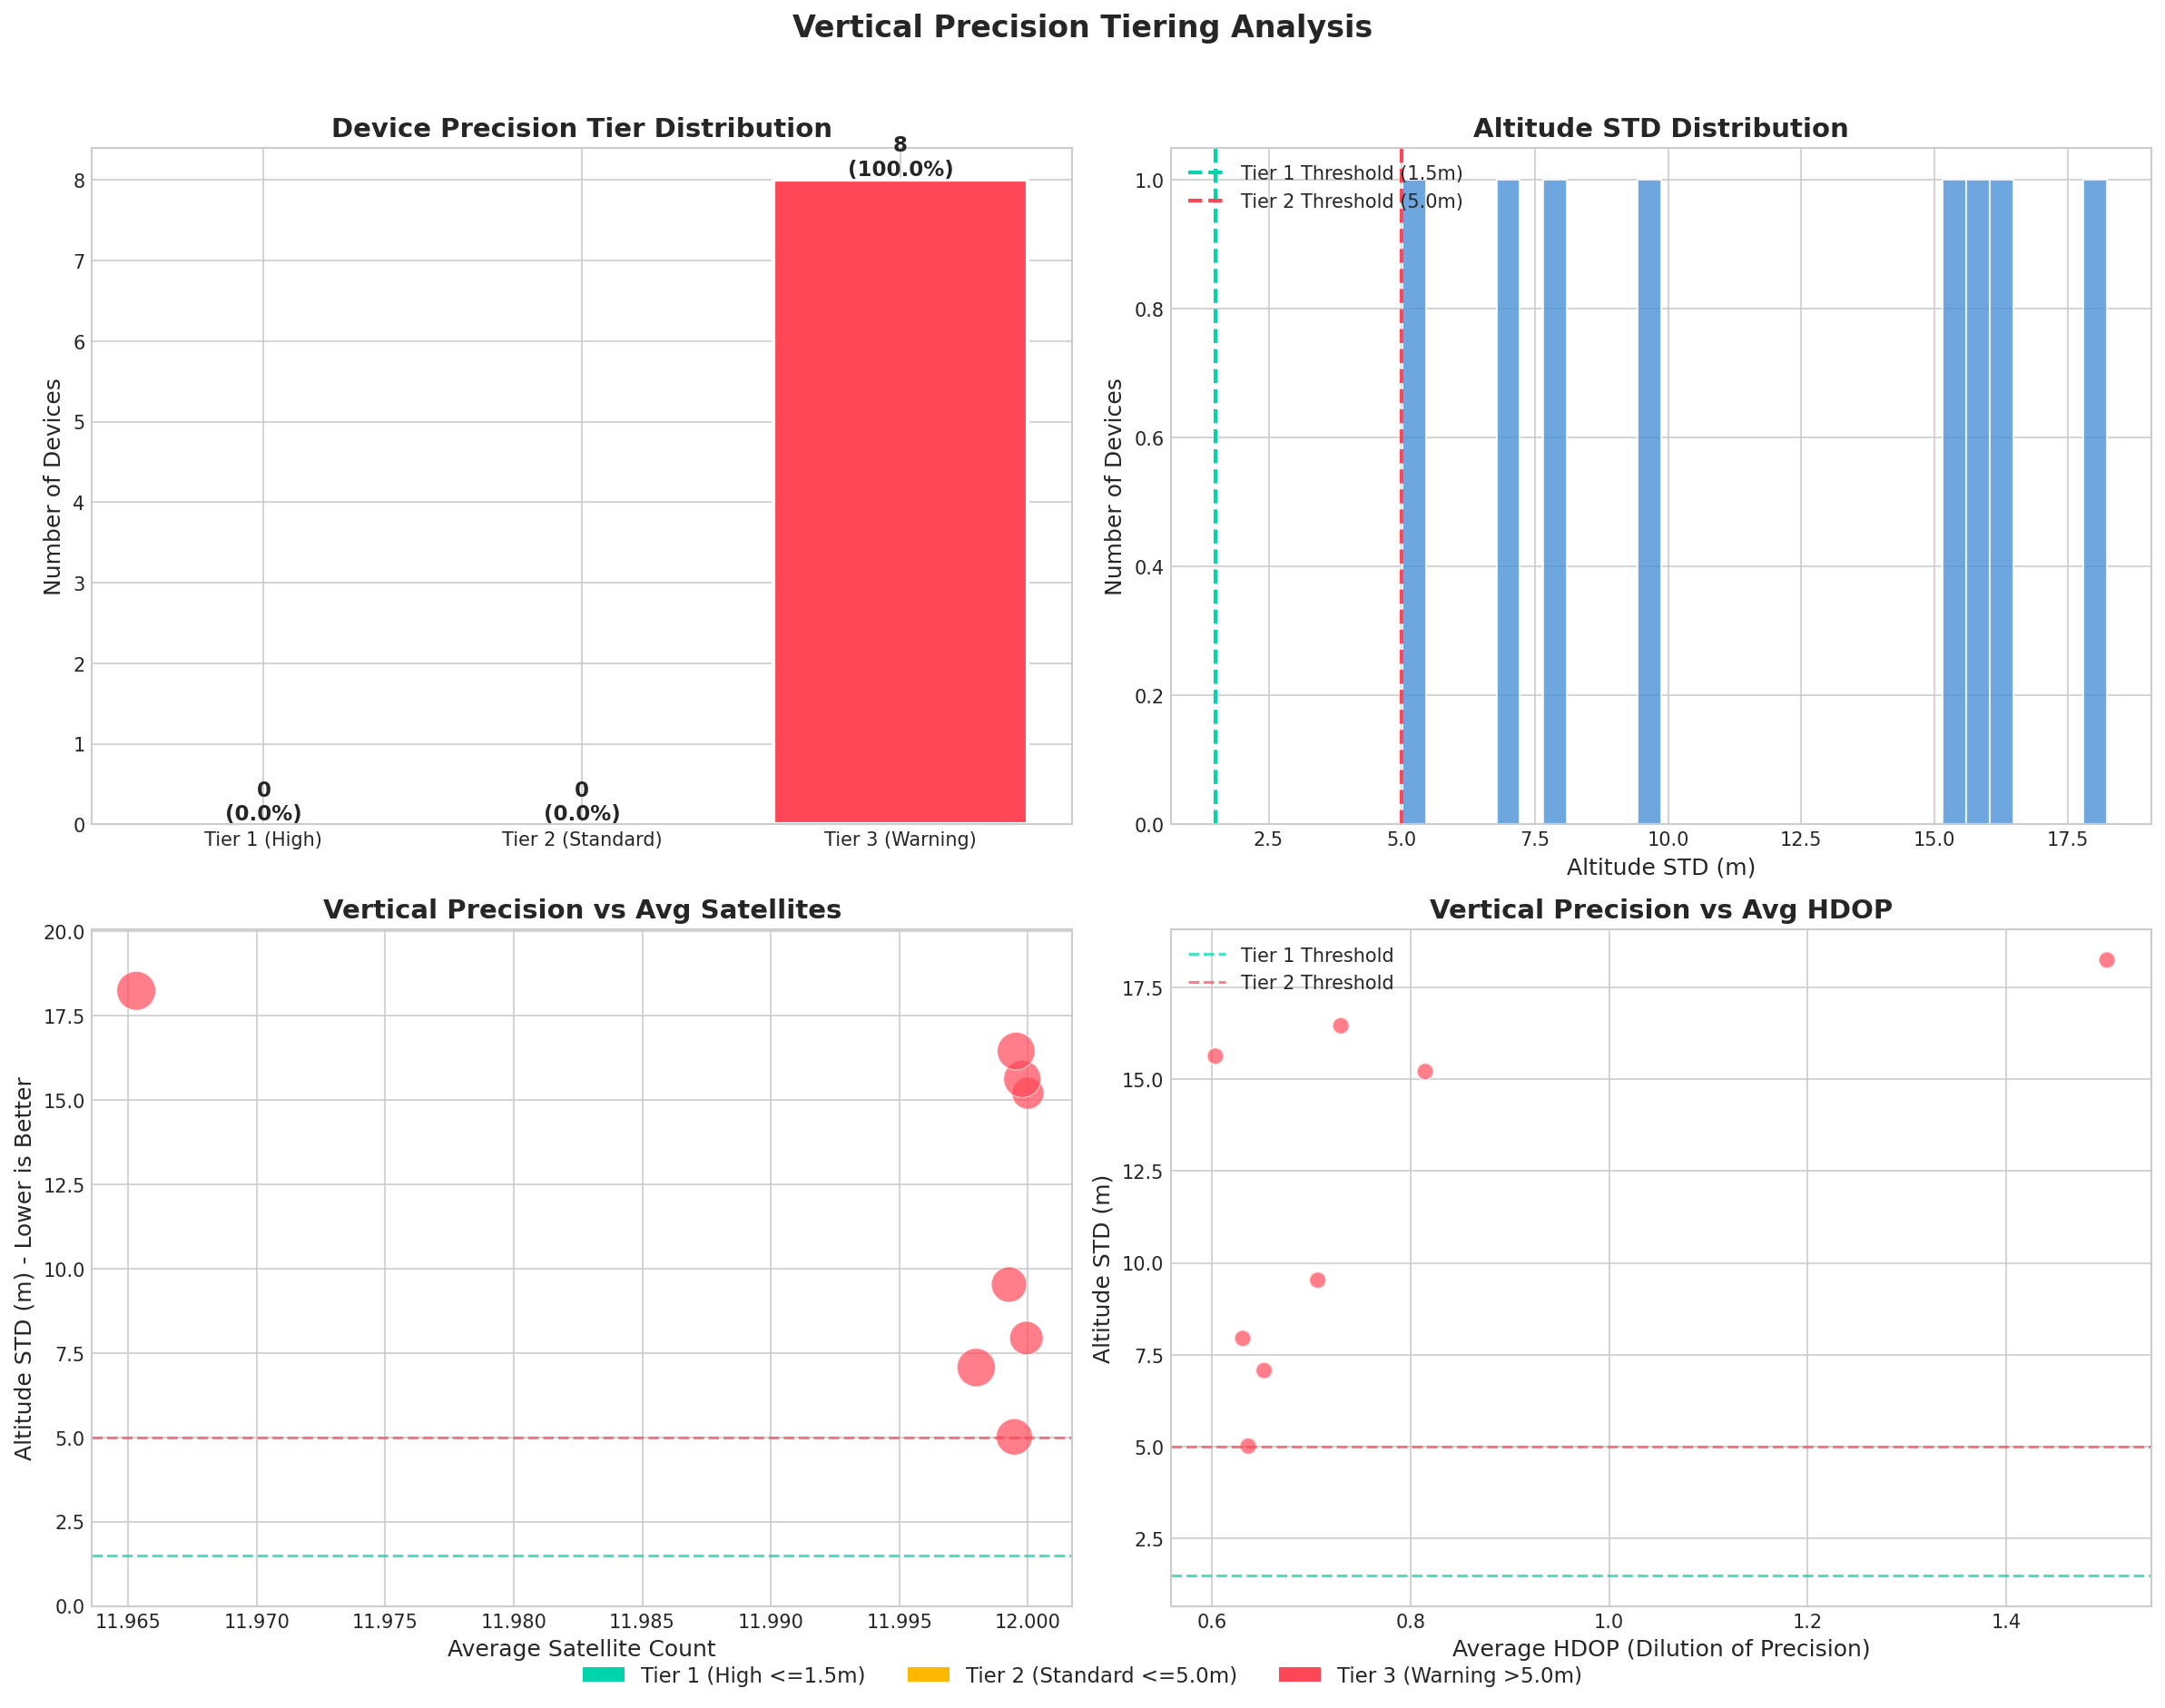
\includegraphics[width=\textwidth]{01_vertical_precision_tiering.png}
    \caption{Vertical Precision Tiering Analysis. Top-left: Device distribution by tier. Top-right: Altitude STD histogram with tier thresholds. Bottom-left: STD vs satellite count relationship. Bottom-right: STD vs HDOP correlation.}
    \label{fig:precision_tiering}
\end{figure}

\subsection{Analysis}

\begin{itemize}
    \item All devices maintain high satellite counts ($\approx$12) and low HDOP values ($<$1.0 for most), yet exhibit poor vertical precision
    \item This decoupling between HDOP and actual precision suggests that traditional DOP metrics may not fully capture vertical accuracy in this deployment
    \item The most stable device (\texttt{9994605977}) achieves STD of 5.01m, just above the Tier 2 threshold
    \item Device \texttt{1878250224} shows significantly higher HDOP (1.50) correlating with worst precision
\end{itemize}

\newpage

% Dimension 2: Environmental Coupling
\section{Dimension 2: Environmental Coupling Analysis}

\subsection{Theoretical Background}

According to the barometric formula, atmospheric pressure $P$ decreases with altitude $h$:

\begin{equation}
P = P_0 \cdot \exp\left(-\frac{Mgh}{RT}\right)
\end{equation}

where $P_0$ is sea-level pressure, $M$ is molar mass of air, $g$ is gravitational acceleration, $R$ is the gas constant, and $T$ is temperature.

For GNSS altitude measurements to be physically consistent, we expect:
\begin{itemize}
    \item \textbf{Strong negative correlation} ($r < -0.5$) between altitude and pressure
    \item Weak or no correlation between altitude and temperature/humidity (unless thermal drift exists)
\end{itemize}

\subsection{Results}

\subsubsection{Global Correlation Matrix (All Devices)}

\begin{table}[H]
\centering
\caption{Environmental Factor Correlation Matrix}
\begin{tabular}{lrrrr}
\toprule
 & \textbf{Altitude} & \textbf{Pressure} & \textbf{Temperature} & \textbf{Humidity} \\
\midrule
Altitude & 1.0000 & \textcolor{tier3}{-0.7258} & -0.0309 & -0.0141 \\
Pressure & -0.7258 & 1.0000 & -0.1553 & -0.1714 \\
Temperature & -0.0309 & -0.1553 & 1.0000 & -0.3215 \\
Humidity & -0.0141 & -0.1714 & -0.3215 & 1.0000 \\
\bottomrule
\end{tabular}
\end{table}

\textbf{Observation:} Global correlation shows $r = -0.7258$ between altitude and pressure, which appears reasonable. However, this is largely driven by altitude differences \textit{between} devices at different locations.

\subsubsection{Single-Device Correlation (Reference Device)}

When analyzing a single device (eliminating location variance):

\begin{table}[H]
\centering
\caption{Reference Device (\texttt{...78250224}) Correlation}
\begin{tabular}{lrrrr}
\toprule
 & \textbf{Altitude} & \textbf{Pressure} & \textbf{Temperature} & \textbf{Humidity} \\
\midrule
Altitude & 1.0000 & \textcolor{tier3}{+0.0465} & -0.0236 & -0.0562 \\
Pressure & +0.0465 & 1.0000 & -0.5407 & -0.4611 \\
Temperature & -0.0236 & -0.5407 & 1.0000 & 0.2994 \\
Humidity & -0.0562 & -0.4611 & 0.2994 & 1.0000 \\
\bottomrule
\end{tabular}
\end{table}

\textbf{Critical Finding:} The single-device altitude-pressure correlation is $r = +0.0465$ (essentially zero), indicating that GNSS altitude variations are \textbf{not tracking actual atmospheric altitude changes}. This is a significant anomaly.

\subsubsection{Per-Device Coupling Strength}

\begin{table}[H]
\centering
\caption{Altitude-Pressure Correlation by Device}
\begin{tabular}{lrrl}
\toprule
\textbf{Device ID} & \textbf{Correlation (r)} & \textbf{Records} & \textbf{Assessment} \\
\midrule
...948226 & -0.022 & 18,462 & Weak (Anomaly) \\
...527426 & +0.023 & 14,185 & Positive (Anomaly) \\
...508217 & +0.033 & 15,971 & Positive (Anomaly) \\
...250224 & +0.046 & 19,682 & Positive (Anomaly) \\
...437779 & +0.058 & 19,039 & Positive (Anomaly) \\
...605977 & +0.096 & 16,925 & Positive (Anomaly) \\
...369164 & +0.104 & 12,913 & Positive (Anomaly) \\
...373510 & \textcolor{tier3}{+0.331} & 17,991 & \textcolor{tier3}{Strong Positive (Severe)} \\
\bottomrule
\end{tabular}
\end{table}

\textbf{Summary:}
\begin{itemize}
    \item Strong coupling devices ($r < -0.5$): \textbf{0}
    \item Weak coupling devices ($r \geq -0.3$): \textbf{8 (100\%)}
\end{itemize}

\subsection{Visualization}

\begin{figure}[H]
    \centering
    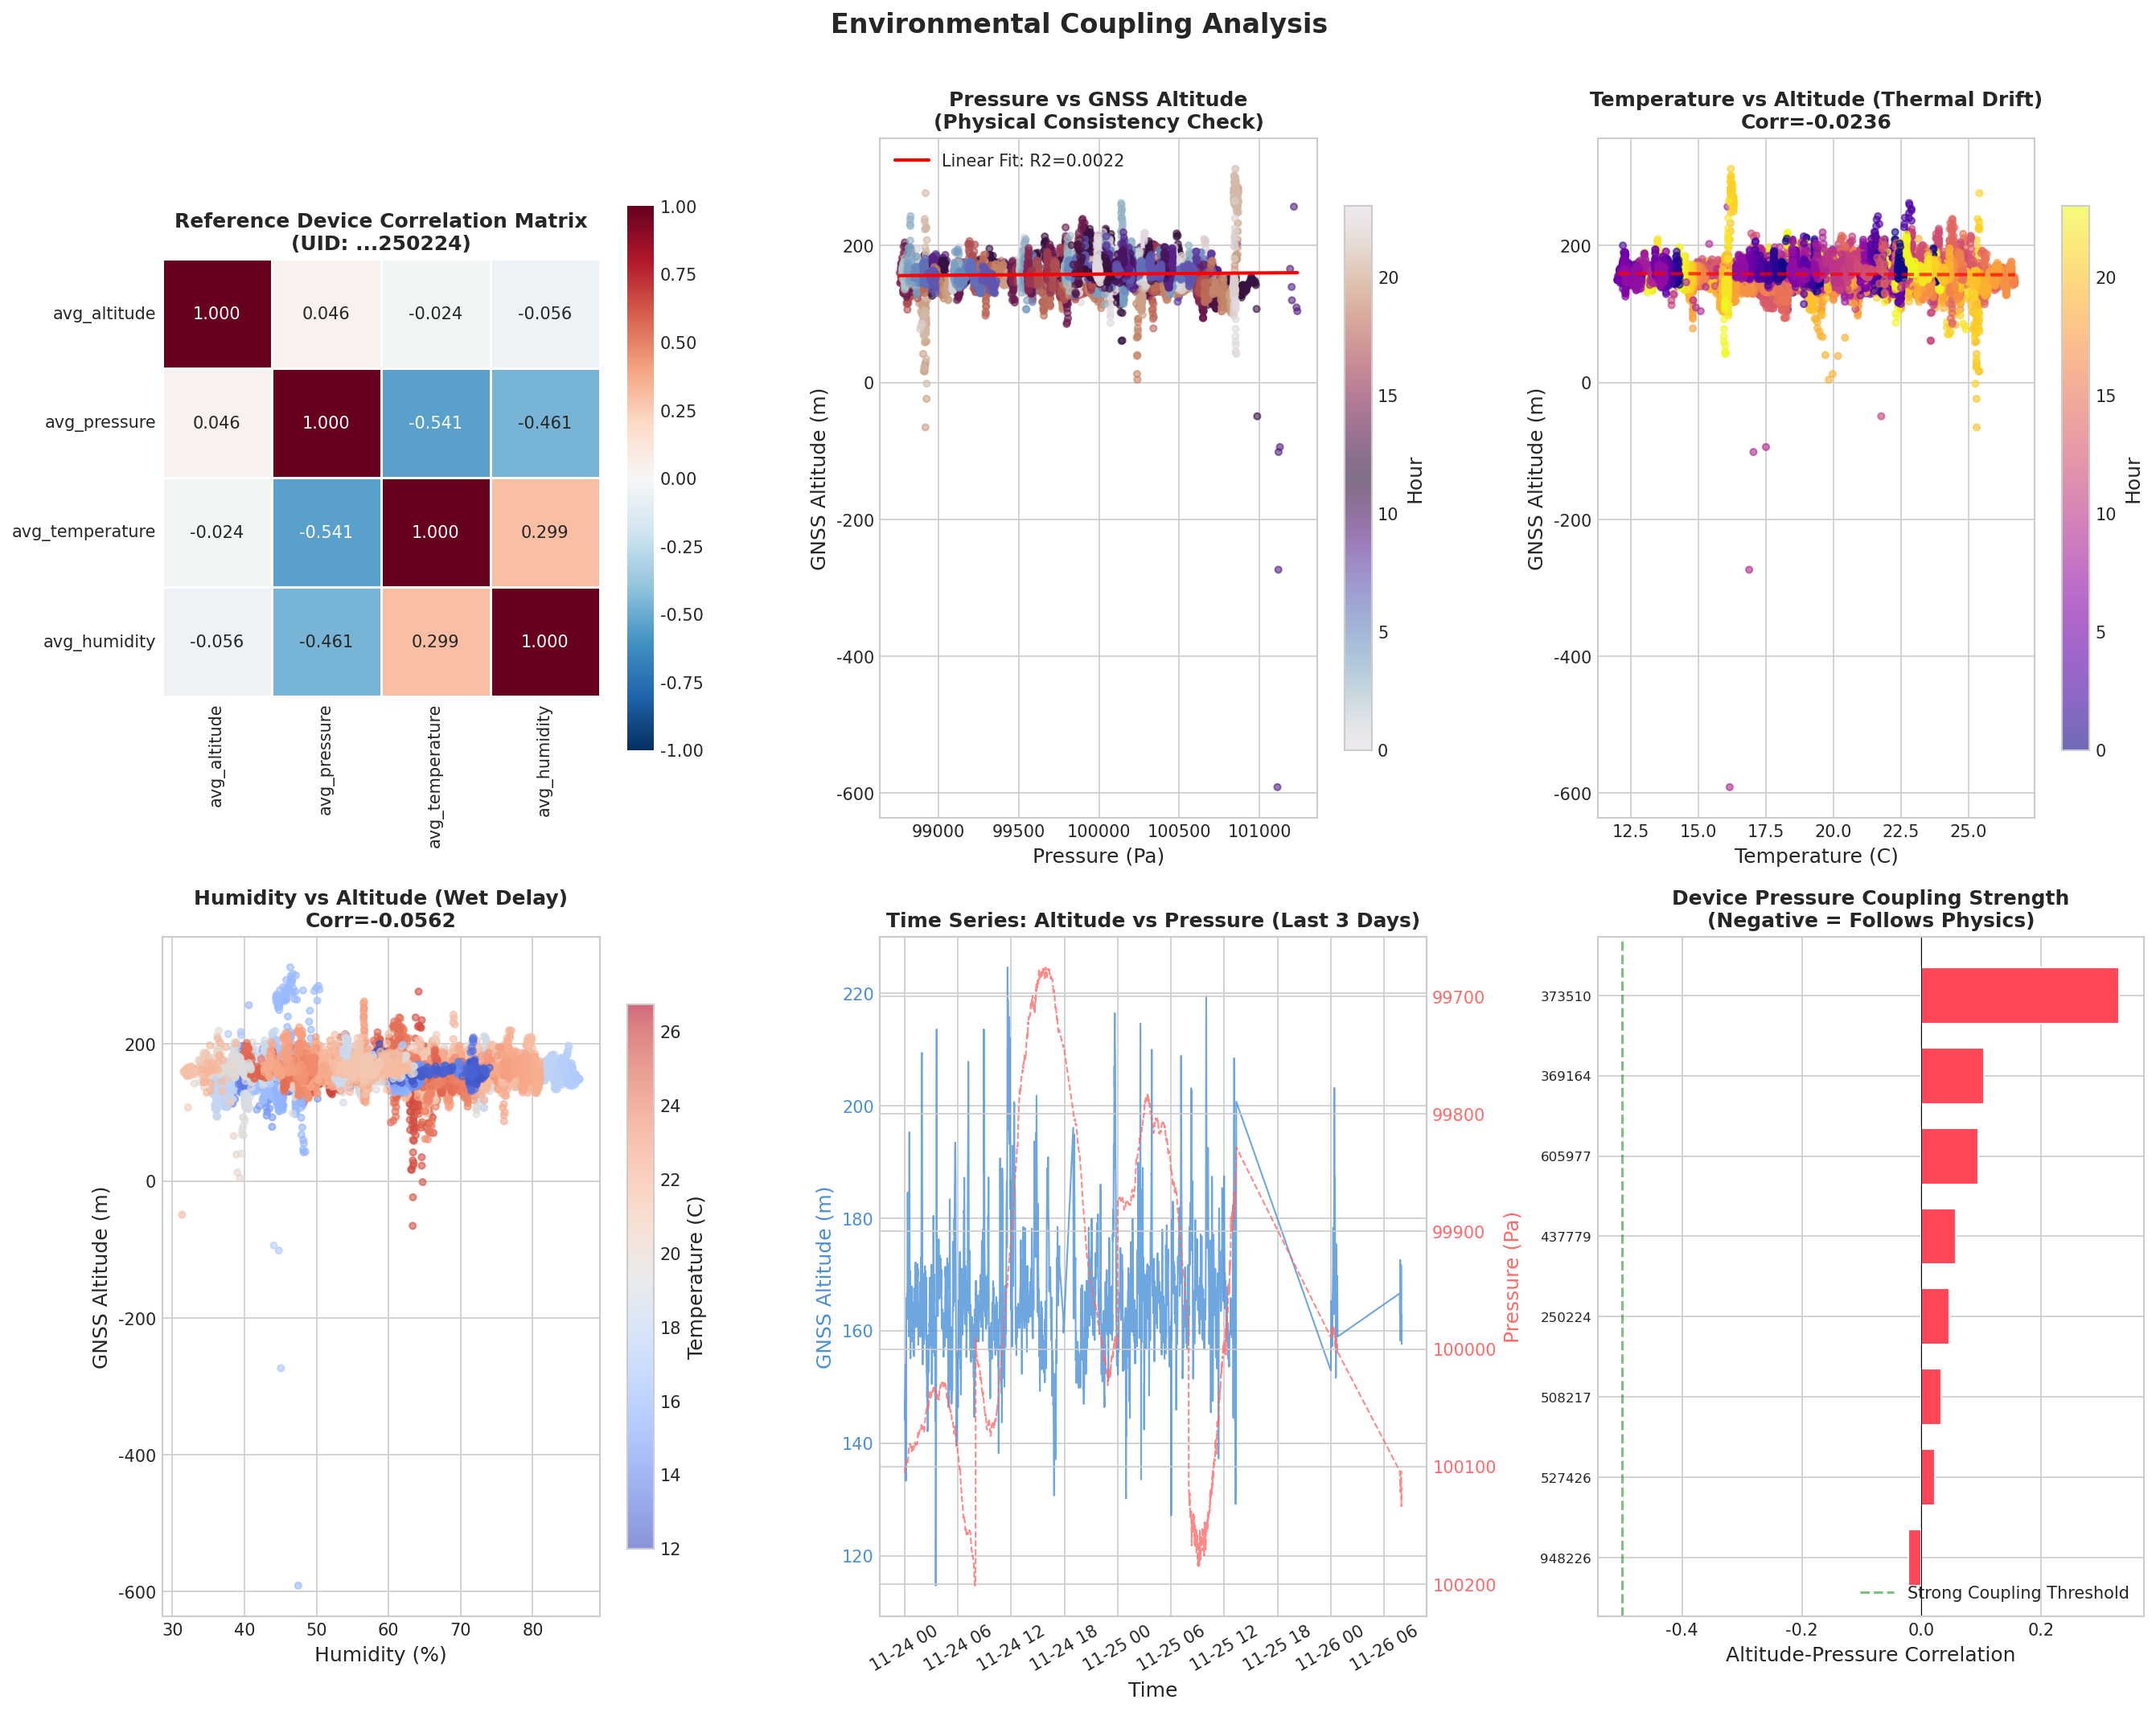
\includegraphics[width=\textwidth]{02_environmental_coupling.png}
    \caption{Environmental Coupling Analysis. Top row: Correlation heatmap, pressure vs altitude scatter with linear fit, temperature vs altitude scatter. Bottom row: Humidity vs altitude, time series comparison, per-device coupling strength.}
    \label{fig:env_coupling}
\end{figure}

\subsection{Interpretation}

The lack of expected negative altitude-pressure correlation within individual devices suggests:

\begin{enumerate}
    \item \textbf{GNSS altitude noise dominates:} Random measurement errors are larger than actual altitude variations
    \item \textbf{Static deployment:} Devices are stationary, so true altitude doesn't vary with weather
    \item \textbf{Sensor decoupling:} The barometric sensor and GNSS receiver may not be physically co-located or time-synchronized
\end{enumerate}

\newpage

% Dimension 3: Diurnal Cycle
\section{Dimension 3: Diurnal Cycle Analysis (Multipath Detection)}

\subsection{Theoretical Background}

Multipath interference occurs when GNSS signals reflect off nearby surfaces (buildings, metal structures, water) before reaching the antenna. This manifests as:

\begin{itemize}
    \item \textbf{24-hour periodicity:} As satellites traverse the sky, reflection geometry changes systematically
    \item \textbf{12-hour sub-harmonic:} Secondary peaks due to GPS orbital period ($\approx$12 hours)
    \item \textbf{Amplitude > 2m:} Significant multipath typically produces meter-level errors
\end{itemize}

\subsection{Results}

\subsubsection{Diurnal Amplitude Comparison}

\begin{table}[H]
\centering
\caption{Diurnal Amplitude: Stable vs Unstable Device}
\begin{tabular}{lrrr}
\toprule
\textbf{Device Category} & \textbf{Device ID} & \textbf{Altitude STD (m)} & \textbf{Diurnal Amplitude (m)} \\
\midrule
Most Stable & ...605977 & 5.01 & \textcolor{tier2}{11.17} \\
Least Stable & ...250224 & 18.24 & \textcolor{tier3}{21.68} \\
\bottomrule
\end{tabular}
\end{table}

\subsubsection{Multipath Risk Assessment}

\begin{table}[H]
\centering
\caption{Multipath Risk Distribution}
\begin{tabular}{lccc}
\toprule
\textbf{Risk Level} & \textbf{Amplitude Threshold} & \textbf{Devices} & \textbf{Percentage} \\
\midrule
\textcolor{tier3}{High Risk} & $>$ 5m & 8 & 100\% \\
\textcolor{tier2}{Medium Risk} & 2--5m & 0 & 0\% \\
\textcolor{tier1}{Low Risk} & $<$ 2m & 0 & 0\% \\
\bottomrule
\end{tabular}
\end{table}

\textbf{Critical Finding:} All devices exhibit high-risk multipath signatures with diurnal amplitudes exceeding 5m.

\subsection{Visualization}

\begin{figure}[H]
    \centering
    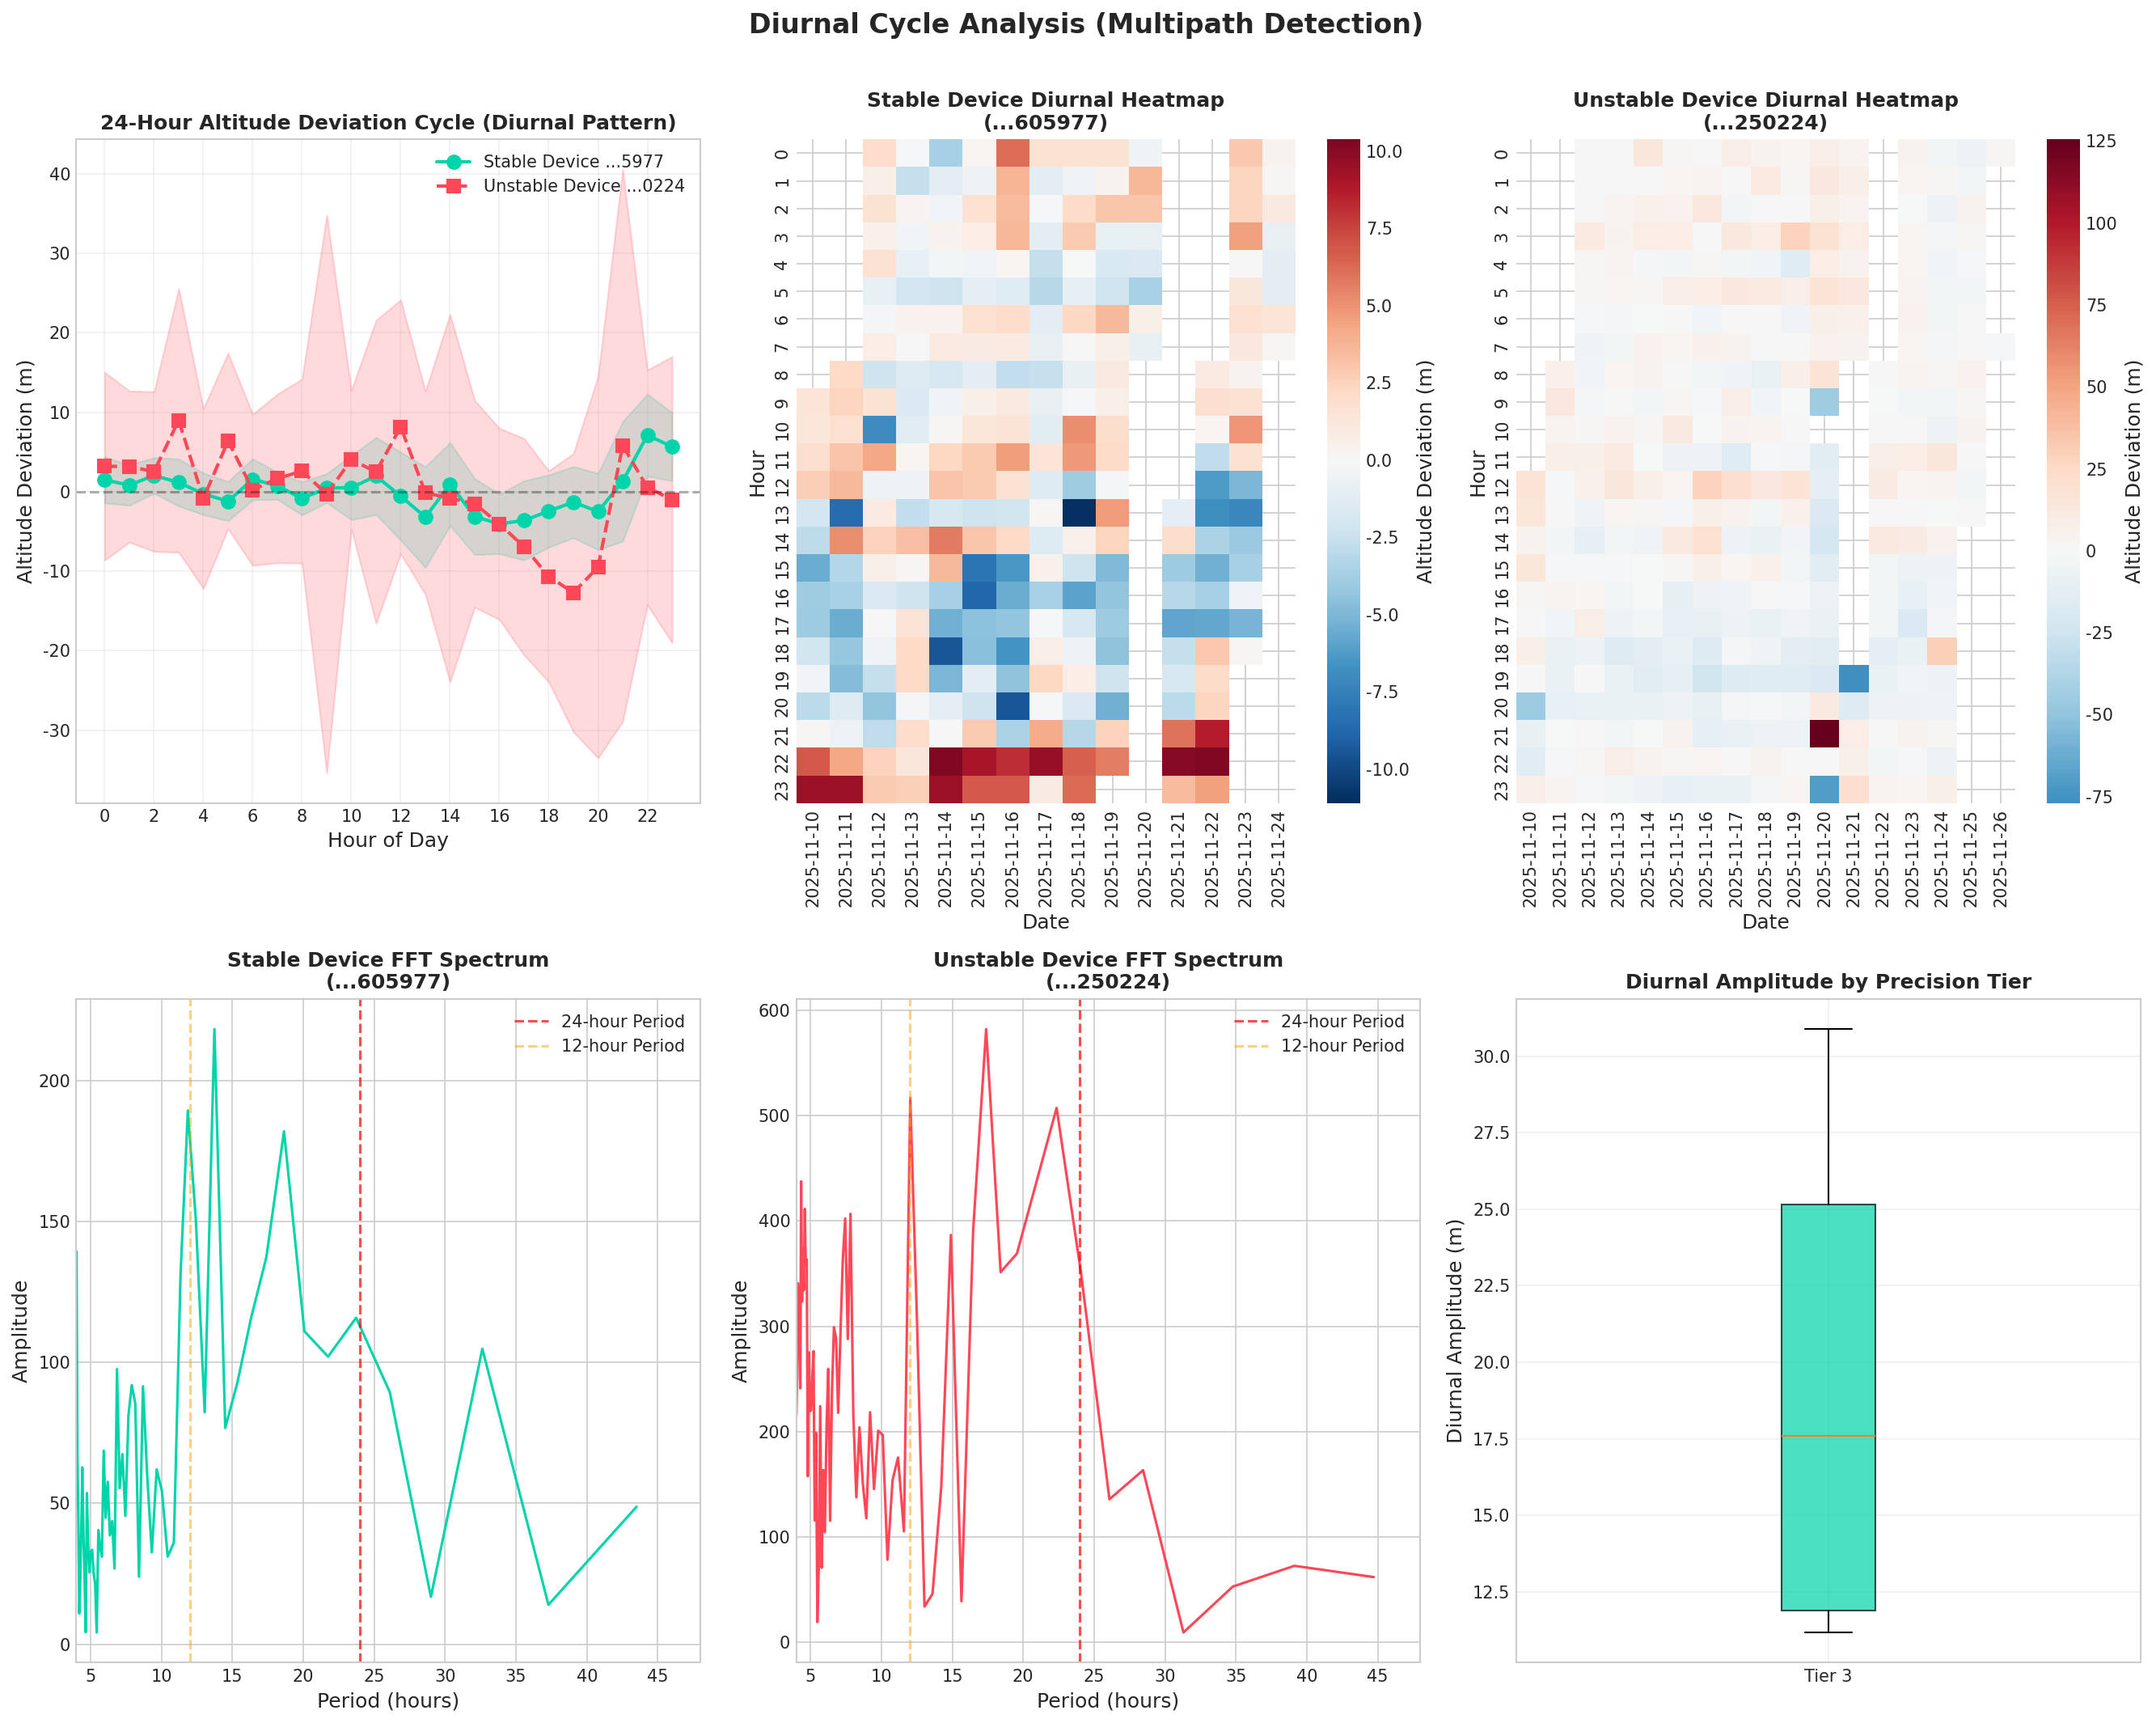
\includegraphics[width=\textwidth]{03_diurnal_cycle_multipath.png}
    \caption{Diurnal Cycle Analysis. Top row: 24-hour altitude deviation pattern comparison, stable device heatmap, unstable device heatmap. Bottom row: FFT spectrum (stable), FFT spectrum (unstable), amplitude distribution by tier.}
    \label{fig:diurnal}
\end{figure}

\subsection{Interpretation}

\begin{enumerate}
    \item \textbf{Systematic 24-hour patterns} are evident in both stable and unstable devices, confirming multipath as a primary error source

    \item \textbf{FFT analysis} reveals strong spectral components at 24-hour and 12-hour periods, consistent with GPS satellite orbital characteristics

    \item \textbf{Even the ``most stable'' device} shows 11.17m diurnal amplitude, indicating that multipath affects the entire deployment

    \item \textbf{Heatmap patterns} show consistent hour-by-hour deviations across multiple days, ruling out random noise
\end{enumerate}

\subsection{Recommended Actions}

\begin{itemize}
    \item Conduct site survey to identify reflective surfaces (metal roofs, glass facades, water features)
    \item Consider antenna relocation or installation of ground planes / choke rings
    \item Implement sidereal filtering to mitigate repeating multipath signatures
    \item Evaluate multi-frequency GNSS receivers for improved multipath rejection
\end{itemize}

\newpage

% Conclusions
\section{Conclusions}

\subsection{Summary of Findings}

\begin{enumerate}
    \item \textbf{Vertical Precision:}
    \begin{itemize}
        \item 100\% of devices classified as Tier 3 (Warning)
        \item Best device: STD = 5.01m; Worst device: STD = 18.24m
        \item One device shows 903m altitude range anomaly requiring investigation
    \end{itemize}

    \item \textbf{Environmental Coupling:}
    \begin{itemize}
        \item All devices show weak or anomalous altitude-pressure correlation
        \item No devices demonstrate expected negative coupling ($r < -0.5$)
        \item GNSS altitude variations appear decoupled from atmospheric physics
    \end{itemize}

    \item \textbf{Multipath Effects:}
    \begin{itemize}
        \item 100\% of devices exhibit high-risk diurnal patterns (amplitude > 5m)
        \item Strong 24-hour and 12-hour periodicities detected via FFT
        \item Systematic multipath interference confirmed across entire deployment
    \end{itemize}
\end{enumerate}

\subsection{Data Quality Assessment}

\begin{table}[H]
\centering
\caption{Overall Data Quality Score}
\begin{tabular}{lcc}
\toprule
\textbf{Metric} & \textbf{Score} & \textbf{Rating} \\
\midrule
Vertical Precision & 0/8 pass Tier 2 & \textcolor{tier3}{Poor} \\
Environmental Coupling & 0/8 strong coupling & \textcolor{tier3}{Poor} \\
Multipath Resistance & 0/8 low risk & \textcolor{tier3}{Poor} \\
\midrule
\textbf{Overall} & & \textcolor{tier3}{\textbf{Poor}} \\
\bottomrule
\end{tabular}
\end{table}

\subsection{Recommendations}

\begin{enumerate}
    \item \textbf{Immediate:} Inspect device \texttt{1878250224} for hardware issues
    \item \textbf{Short-term:} Survey all antenna installation sites for multipath sources
    \item \textbf{Medium-term:} Implement RTK/PPP corrections or relocate antennas
    \item \textbf{Long-term:} Consider upgrading to multi-frequency GNSS with better multipath mitigation
\end{enumerate}

\newpage

% Appendix
\appendix
\section{Appendix: Data Files}

The following output files are available in the \texttt{data/reports/deep\_analysis/} directory:

\begin{table}[H]
\centering
\begin{tabular}{ll}
\toprule
\textbf{File} & \textbf{Description} \\
\midrule
\texttt{device\_tier\_stats.csv} & Complete device statistics with tier classification \\
\texttt{device\_coupling\_analysis.csv} & Per-device environmental coupling coefficients \\
\texttt{diurnal\_amplitude\_analysis.csv} & Diurnal amplitude measurements by device \\
\texttt{01\_vertical\_precision\_tiering.png} & Precision tiering visualization \\
\texttt{02\_environmental\_coupling.png} & Environmental coupling analysis plots \\
\texttt{03\_diurnal\_cycle\_multipath.png} & Diurnal cycle and multipath analysis \\
\bottomrule
\end{tabular}
\end{table}

\section{Appendix: Methodology Notes}

\subsection{Tier Classification}
Devices are classified based on the standard deviation of their altitude measurements over the observation period. Thresholds are based on typical GNSS performance expectations:
\begin{itemize}
    \item Tier 1 ($\leq$1.5m): Achievable with RTK/PPK or high-quality single-point positioning
    \item Tier 2 ($\leq$5.0m): Standard single-point GNSS performance
    \item Tier 3 ($>$5.0m): Indicates environmental issues or hardware problems
\end{itemize}

\subsection{Correlation Analysis}
Pearson correlation coefficients are computed between altitude and environmental factors. Strong negative altitude-pressure correlation is expected based on the barometric altitude formula.

\subsection{FFT Analysis}
Fast Fourier Transform is applied to detrended hourly altitude data to identify periodic components. A 24-hour rolling mean is subtracted to remove long-term trends before spectral analysis.

\end{document}
